\documentclass[tikz,border=8pt]{standalone}
% Shared look for every TikZ diagram. Load with \input{../../tools/tikz-style.tex}
\usepackage[sfdefault]{roboto}
\usetikzlibrary{arrows.meta, positioning, shapes.geometric, calc, fit, backgrounds}
\definecolor{cblue}{HTML}{4C78A8}
\definecolor{corange}{HTML}{F58518}
\definecolor{cgreen}{HTML}{54A24B}
\definecolor{cred}{HTML}{E45756}
\definecolor{cpurple}{HTML}{B279A2}
\definecolor{cgrey}{HTML}{6B6B6B}
\tikzset{
  every picture/.style={font=\sffamily, line width=1.2pt},
  box/.style={draw=#1, fill=#1!12, rounded corners=4pt, align=center, inner sep=7pt, minimum height=1.1cm},
  box/.default=cgrey,
  arrow/.style={-{Stealth[length=3mm]}, draw=cgrey, line width=1.4pt},
  title/.style={font=\sffamily\bfseries\Large},
  note/.style={font=\sffamily\small, text=cgrey, align=center},
}
\AtBeginDocument{\hyphenpenalty=10000 \exhyphenpenalty=10000}

% The gap this Note fills. The route of the graph-search Notes (3.414 m, cell centres as dots) moves a point from
% cell to cell. The robot is a disk of radius 0.25 m centred on the middle of its axle, facing 30 degrees: placing
% it takes its centre (x, y) and its heading theta.
\begin{document}
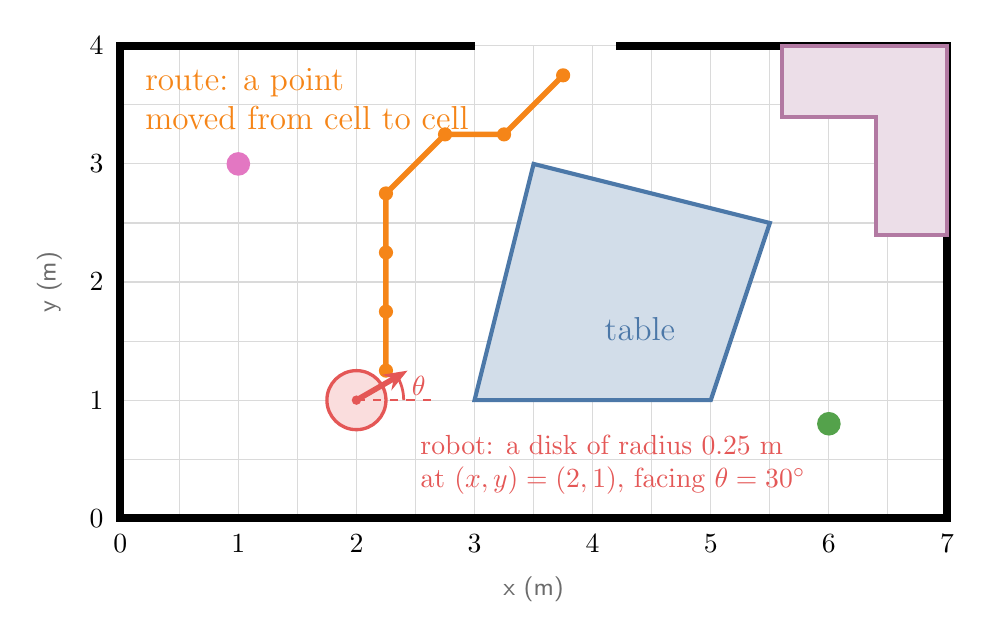
\begin{tikzpicture}[scale=1.5, every node/.append style={font=\large}]
  \definecolor{cpink}{HTML}{E377C2}
  \draw[cgrey!25, line width=0.4pt] (0,0) grid[step=0.5] (7,4);
  \draw[black, line width=3pt] (3.0,4) -- (0,4) -- (0,0) -- (7,0) -- (7,4) -- (4.2,4);
  \filldraw[cblue!25, draw=cblue, line width=1.5pt] (3,1) -- (5,1) -- (5.5,2.5) -- (3.5,3) -- cycle;
  \node[cblue] at (4.4,1.6) {table};
  \filldraw[cpurple!25, draw=cpurple, line width=1.5pt] (5.6,4) -- (5.6,3.4) -- (6.4,3.4) -- (6.4,2.4) -- (7,2.4) -- (7,4) -- cycle;
  \fill[cpink] (1,3) circle (0.1);
  \fill[cgreen] (6,0.8) circle (0.1);
  % the route through cell centres
  \draw[corange, line width=2pt] (2.25,1.25) -- (2.25,1.75) -- (2.25,2.25) -- (2.25,2.75) -- (2.75,3.25) -- (3.25,3.25) -- (3.75,3.75);
  \foreach \p in {(2.25,1.25),(2.25,1.75),(2.25,2.25),(2.25,2.75),(2.75,3.25),(3.25,3.25),(3.75,3.75)}
    \fill[corange] \p circle (0.06);
  \node[corange, anchor=north west, align=left] at (0.12,3.9) {route: a point\\ moved from cell to cell};
  % the robot
  \filldraw[cred, fill=cred!20, line width=1.2pt] (2,1) circle (0.25);
  \draw[-{Stealth[length=3mm]}, cred, line width=2pt] (2,1) -- ++(30:0.5);
  \fill[cred] (2,1) circle (0.04);
  \draw[cred, dashed, line width=0.8pt] (2,1) -- (2.7,1);
  \draw[cred, line width=1pt] (2.4,1) arc (0:30:0.4) node[pos=0.6, right, font=\normalsize] {$\theta$};
  \node[cred, anchor=west, align=left, font=\normalsize] at (2.45,0.45) {robot: a disk of radius 0.25 m\\ at $(x, y) = (2, 1)$, facing $\theta = 30^\circ$};
  \foreach \t in {0,...,7} \node[below, font=\normalsize] at (\t,-0.05) {\t};
  \foreach \t in {0,...,4} \node[left, font=\normalsize] at (-0.05,\t) {\t};
  \node[note] at (3.5,-0.6) {x (m)}; \node[note, rotate=90] at (-0.6,2) {y (m)};
\end{tikzpicture}
\end{document}
